%\VignetteIndexEntry{Tides: characteristics of tidal water level time series.}

\documentclass[10pt,a4wide]{article}
\usepackage{graphicx}
\usepackage{lscape}
\usepackage{bm}
\usepackage{amsmath}
\usepackage{natbib}
\usepackage{Rd}
\usepackage{xcolor}

\author{Tom Cox}
\title{Tides: characteristics of tidal water level time series.}

\usepackage{Sweave}
\begin{document}
\Sconcordance{concordance:Tides.tex:/home/tom/projecten/RPackages/GitHub/Tides/vignettes/Tides.Rnw:%
1 14 1 1 0 2 1 1 4 10 1 2 4 34 1 1 30 1 3 101 1 2 3 11 1}


\maketitle
\section{Intro}
The package was written for the specific purpose of analysing recordings of water levels in intertidal ecosystems. It contains routines to calculate ecologically relevant properties such as the high and low water levels, the inundation frequency at a certain level, average inundation time and height, etc. The main function in the package is the function \texttt{TidalCharacteristics()}.

The core of this function is the function \texttt{extrema()}, an algorithm to calculate the multiple maxima and minima of quasi periodic time series. This note contains a short explanation of how the algorithm works, and explains the different parameters that control its use.

\section{Typical water level time series}
Figure \ref{Fig1} shows a typical water level time series, recorded in 2007 in the Lippenbroek study site \citep{Cox2006, Maris2007}. The grey line corresponds to the ground level at the data logger. This data set has several typical features of such water level time series. The first part of the graph shows regular inundation (mark that the average tidal cycle has a period of 12.4h), although the site is not inundated at the 12th tidal cycle. After this period with regular inundations follows a period without inundations; ground water level is steadily decreasing. Next follows another regular period, but after the third cycle, the site does not drain completely, and it stays inundated for 3 consecutive cycles. The last period is again a dry period with decreasing ground water levels.

\begin{figure}[h]
\begin{center}
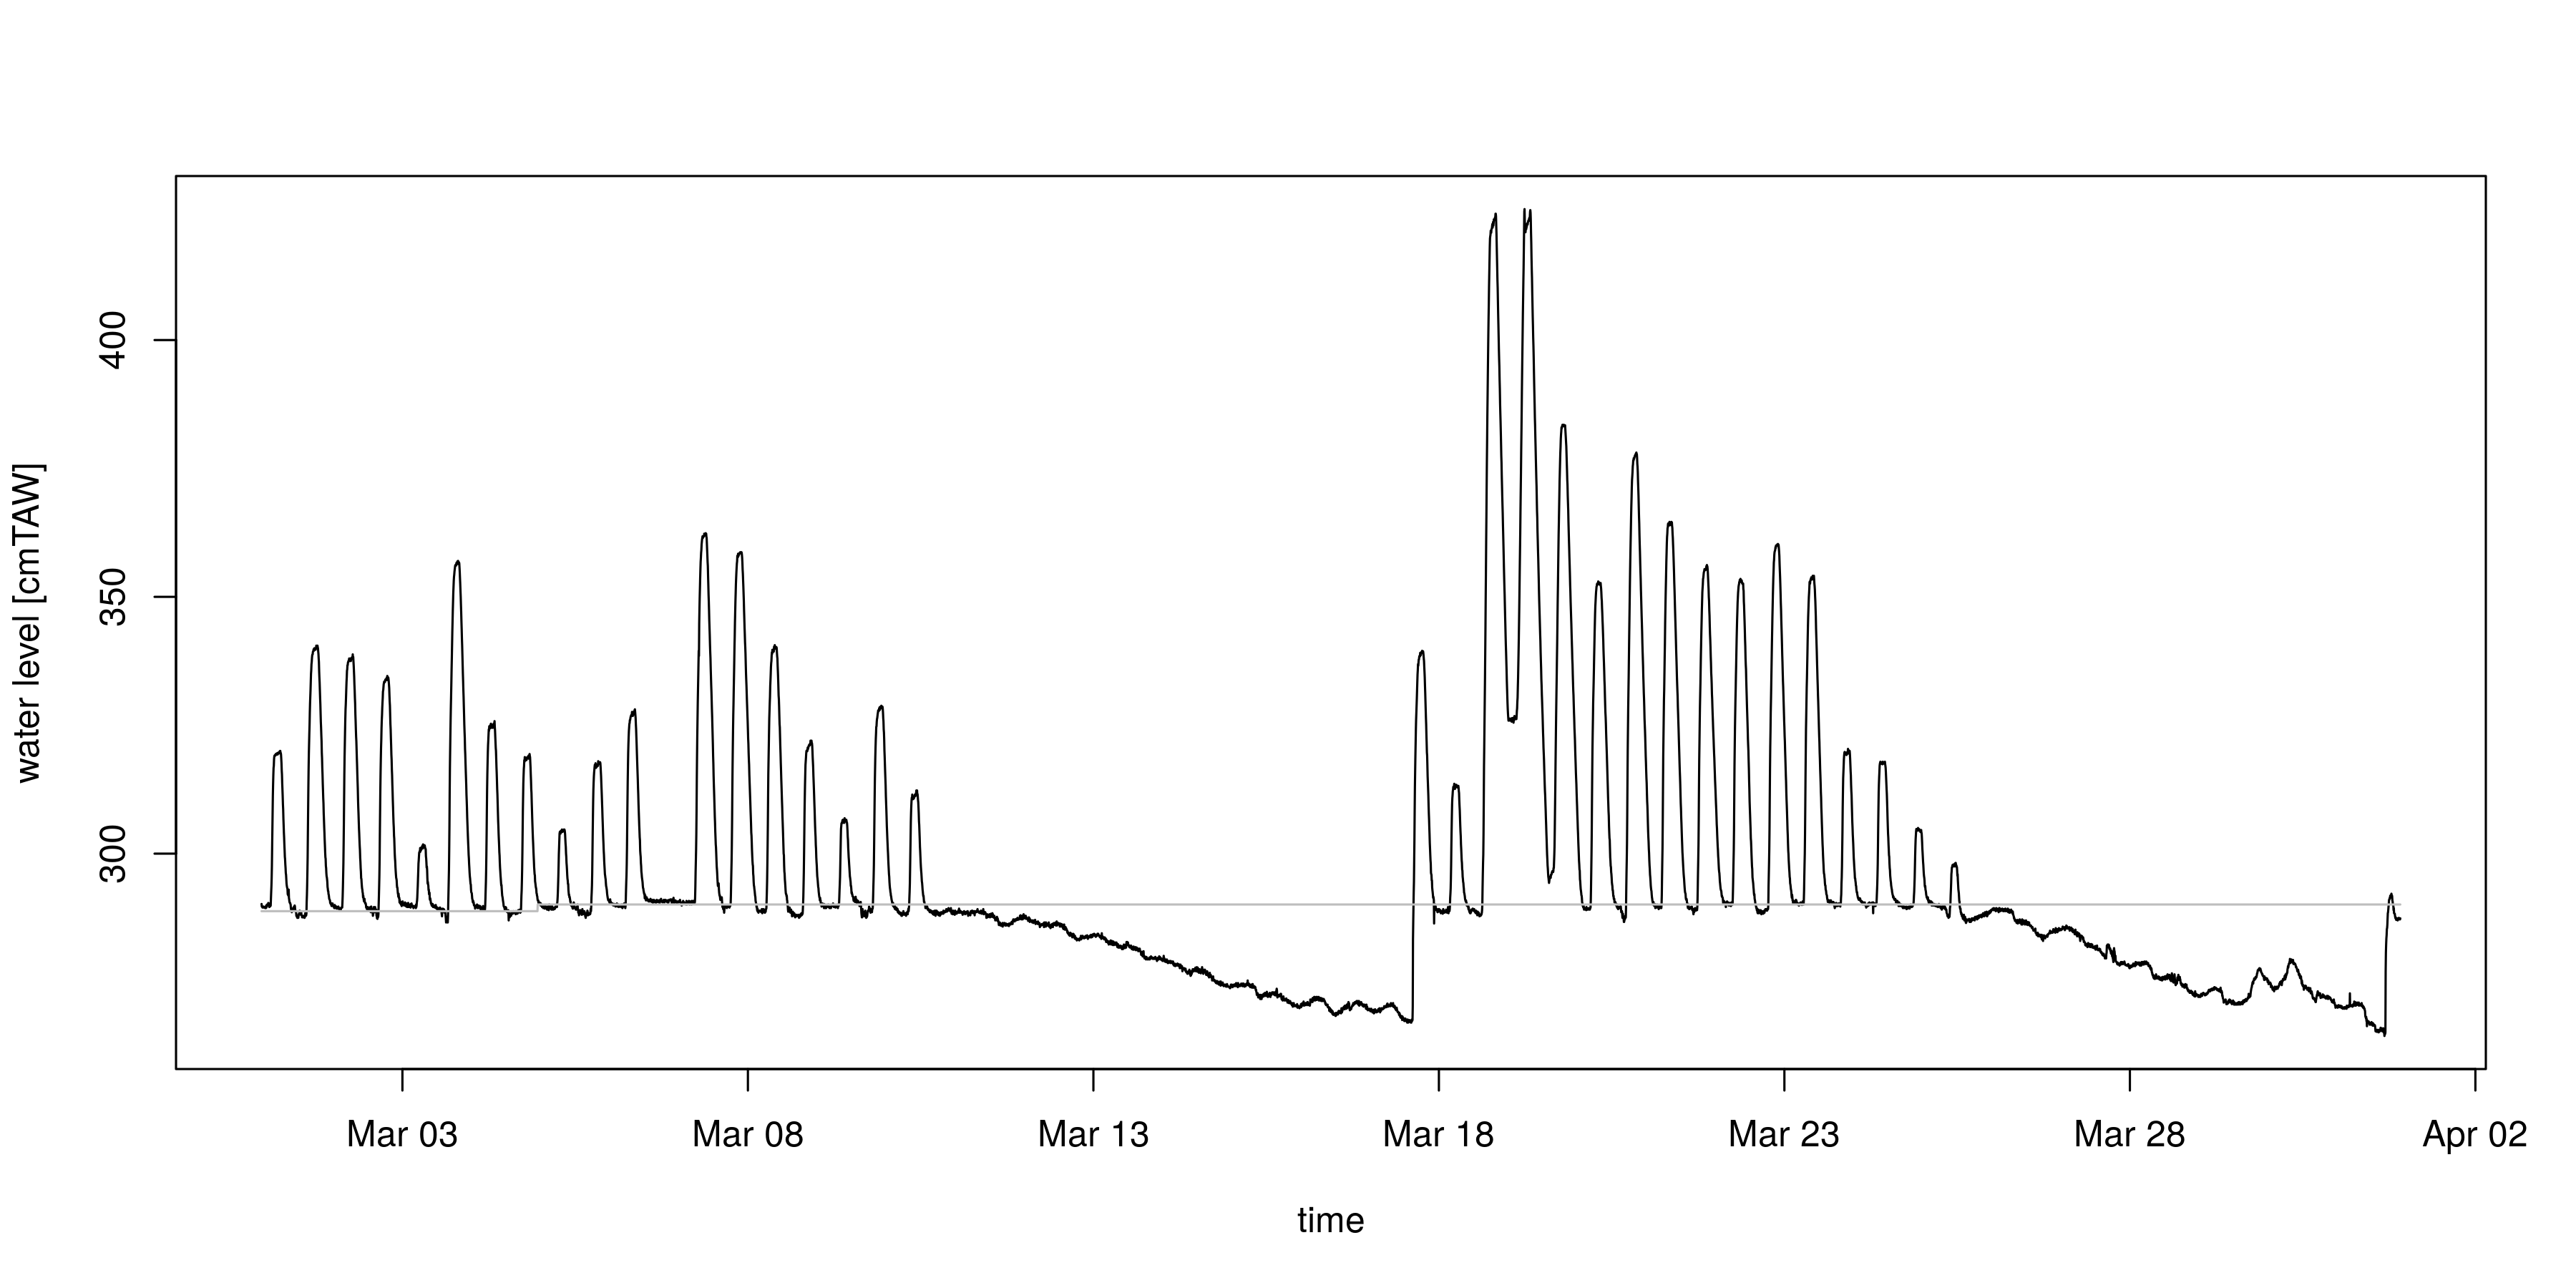
\includegraphics{Tides-TideFig1}
\end{center}
\caption{Typical water level time series} 
\label{Fig1}
\end{figure}


The quantities that are relevant from an ecological perspective are the statistics of inundation time and height (average, standard distribution, maximum, distribution), the relation between these two variables, and the inundation frequency of the site (the proportion of tidal cycles that effectively flood the site). A more formal description of these quantities can be found in \citep{Cox2006}.

The main job to be done is finding all 'maxima' of the time series. If the time difference between two consecutive maxima would be (fairly) constant, this could easily be done by breaking up the time series in time intervals of constant length, and finding the maximum (and minimum) in each interval. However, in the case of tidal water level time series, the interval between consecutive maxima is variable, to the extent that certain fixed time intervals would contain two consecutive maxima. As a result, this simple approach would result in missing the lowest of the two maxima in those intervals. 

\section{Finding the extrema of quasi periodic (water level) time series}
We assume that the time difference between two consecutive maxima is always larger than $T_{min}$. An observed water level\footnote{Although we use the 'water level' terminology throughout, the algorithm can also be useful for other quasi periodic time series} at a certain time is then part of a high water phase, when it is higher than the water levels at time $T_{min}/2$ later and earlier (Figure \ref{Fig2}), or
\begin{align}
h(t) \textrm{ is part of } 	& \textrm{a high water phase} \nonumber\\
\nonumber 			&\Leftrightarrow \\\nonumber
h(t-\frac{T_{min}}{2}) < 	&h(t) > h(t+\frac{T_{min}}{2}) 
\end{align}
All maxima of the time series are then found by determining the maximum for each high water phase.

If the time series is smooth, this algorithm will also work smoothly. Unfortunatly, observed water levels always feature small fluctuations. In such cases, the algorithm will generate spurious maxima in the low water phase. Two different approaches can be taken to deal with such fluctuations. First,  a small offset value could be defined (\texttt{hoffset}), such that an observed water level is part of the high water phase only when it is higher than the water levels at time $T_{min}/2$ later and earlier \emph{plus} the offset value: 

\begin{align}
h(t-\frac{T_{min}}{2}) + \texttt{hoffset}   < 	&h(t) >   h(t+\frac{T_{min}}{2}) + \texttt{hoffset}
\end{align}

The trade-off is that we loose the genuine high waters that are smaller than the offset value.

Alternatively the observed data could be filtered to remove small fluctuations. A movering average with width \texttt{filtconst} is used: \begin{verbatim}filter(h$h,rep(1/filtconst,filtconst))\end{verbatim}

Also here, the trade-off is that some genuine high waters will be lost. Also, during long low water phases  (spanning multiple times T2) with a quasi constant water level and only random fluctuations, such filtering step will not prevent potential spurious maxima generation.

Both approaches are implemented in \texttt{extrema()}.

\begin{figure}[h]
\begin{center}
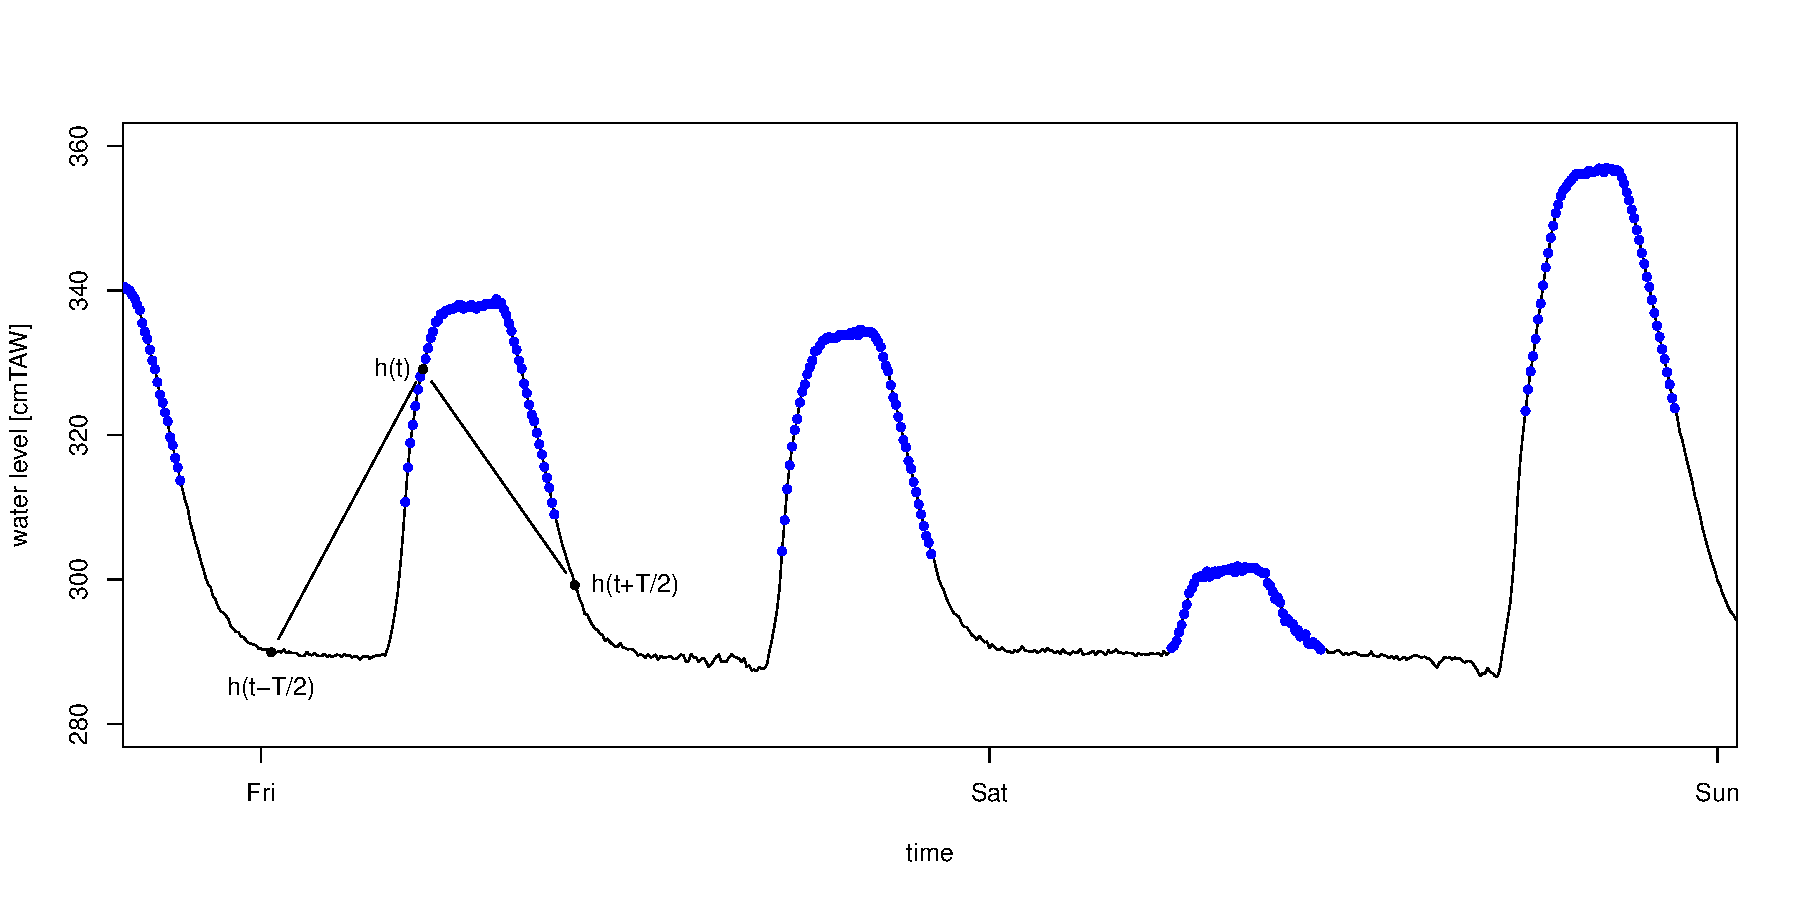
\includegraphics{Tides-TideFig2}

\end{center}
\caption{Determination of the high water phase (blue dots) of the water level time series. A water level is part of a high water phase, when it is higher than the water levels at time $T_{min}/2$ later and earlier} 
\label{Fig2}
\end{figure}




\section{The function \texttt{extrema()}}
The function \texttt{extrema()} performs the calculations described in the previous paragraph. It is the core of \texttt{TidalCharacteristics()}, which is more convenient as it returns further analysed and interpreted output, and is described in the following paragraph. 

\begin{Usage}
\begin{verbatim}extrema(h, h0, T2 = 5*60*60, hoffset = 0, filtconst = 1)\end{verbatim}
\end{Usage}
\begin{Arguments}
\begin{ldescription}
\item[\code{h }] Water level time series. data frame with time and h column
\item[\code{h0 }] Reference level, either single valued vector with dimension corresponding to h
\item[\code{T2 }] 'Lower' bound on half the quasi period, but higher than expected stagnant phase; default = 5h
\item[\code{hoffset}] Offset level, to prevent spurious maxima generation due to small fluctuations. Default = 0 (no offset).
\item[\code{filtconst }] Filtering constant for smoothing the time series with moving average filter. default = 1 (no smoothing)
\end{ldescription}
\end{Arguments}
\begin{Value}
a list containing:
\begin{ldescription}
\item[\code{HL }] Data frame with extrema
\item[\code{h }] original water level data frame with additional attributes
\end{ldescription}
\end{Value}

\section{The function \texttt{TidalCharacteristics()}}
The function \texttt{TidalCharacteristics()} returns further interpreted results: the inundation frequency and the number of inundations during the time span, the average inundation height, the average and maximum inundation time,the average and maximum dry time, and the total time span of observations expressed as number tidal cycles.

As an additional feature, the function also works on time series containing gaps, i.e. periods for which no water level data exist. This is performed by defining a maximum time interval \texttt{dtMax} between consecutive measurements of a continuous observation. When the time interval between two consecutive data points is bigger than \texttt{dtMax} this is considered a gap in the observations. For example, the inundation frequency is then calculated as the number of inundation devided by the total number of tides \emph{during the period for which observations are available}.

\texttt{TidalCharacteristics()} in fact returns an object of class \texttt{Tides}, with an associated simple plotting method. See examples. 
\begin{Usage}
\begin{verbatim}TidalCharacteristics(h,h0 = h$h0,T2 = 5*60*60, hoffset = 0, filtconst = 1, 
                     dtMax = 15,unit = "mins", Tavg = 12.4*60,
                     removegaps = c("All", "Split", "None")) 
TC <- TidalCharacteristics(h,...)\end{verbatim}
\end{Usage}
\begin{Arguments}
\begin{ldescription}
\item[\code{h, h0, T2, hoffset, filtconst }] See description of \texttt{extrema()}
\item[\code{dtMax}] Maximum accepted time interval in a continuous series. Bigger time intervals are considered to be gaps
\item[\code{unit}] Unit of dtMax, Tavg
\item[\code{Tavg}] Average time difference between consecutive maxima in the time series, used to calculate inundation frequency.
\item[\code{removegaps}}] Method to remove gaps in time series from inundation times and dry times
\end{ldescription}
\end{Arguments}
\begin{Value}
An object of class \code{Tides}, i.e. a list containing:
\begin{ldescription}
\item[\code{HL }] Data frame with extrema
\item[\code{h }] original water level data frame with additional attributes
\item[\code{gaps}] a data frame containing start and end times of gaps in the series
\item[\code{IF}] inundation frequency of the reference level
\item[\code{ITs}] inundation times at the reference level
\item[\code{DTs}] dry times at the reference level
\item[\code{h0}] reference level
\item[\code{N}] Total number of cycles in time span
\end{ldescription}
\end{Value}

\section{Examples}
\texttt{waterlevels} is the time series shown in Figure \ref{Fig1}, and is included in the package \texttt{Tides}. Simply applying \texttt{TidalCharacteristics} on \texttt{waterlevels} prints the characteristics of the time series.
\begin{verbatim}
> require(Tides)
> TidalCharacteristics(waterlevels, hoffset=3)
Inundation frequency:  57.62712 
Inundations during time span:  34 
Average inundation height:  50.45294 
Average inundation height (per cycle):  29.07458 
Average inundation time:  425 mins 
Average inundation time (per cycle):  230.5085 mins 
Maximal inundation time:  2050 mins 
Average dry time:  947.7273 mins 
Average dry time (per cycle):  530.0847 mins 
Maximal dry time:  10245 mins 
Average high water:  340.2471 
Average low water:  290.9743 
Time span:  59 average (tidal) cycles 
There were no gaps in the time series
Warning message:
In gapsts(wet$time, dtMax, unit = unit, shiftbegin = TRUE) :
  First data point is beginning of gap. To shift t0, dt is estimated from next continuous series
\end{verbatim}
\textcolor{green}{ADD some explanation about the warning message??}


The resulting object is of class \texttt{Tides}, for which a simple plotting method exist. 

\begin{verbatim}
> TC <- TidalCharacteristics(waterlevels, hoffset=3)
> plot(TC)
\end{verbatim}
The resulting plot is shown in figure \ref{Fig3}. Mark that no maximum is generated at the 12th tidal cycle, with the default values of the filtering (i.e. an offset value of 3 cm and no filtering). When the function would be applied with \texttt{hoffset=0} and \texttt{filtconst=50} there would be a maximum detected during this period.
\begin{figure}[h]
\begin{center}
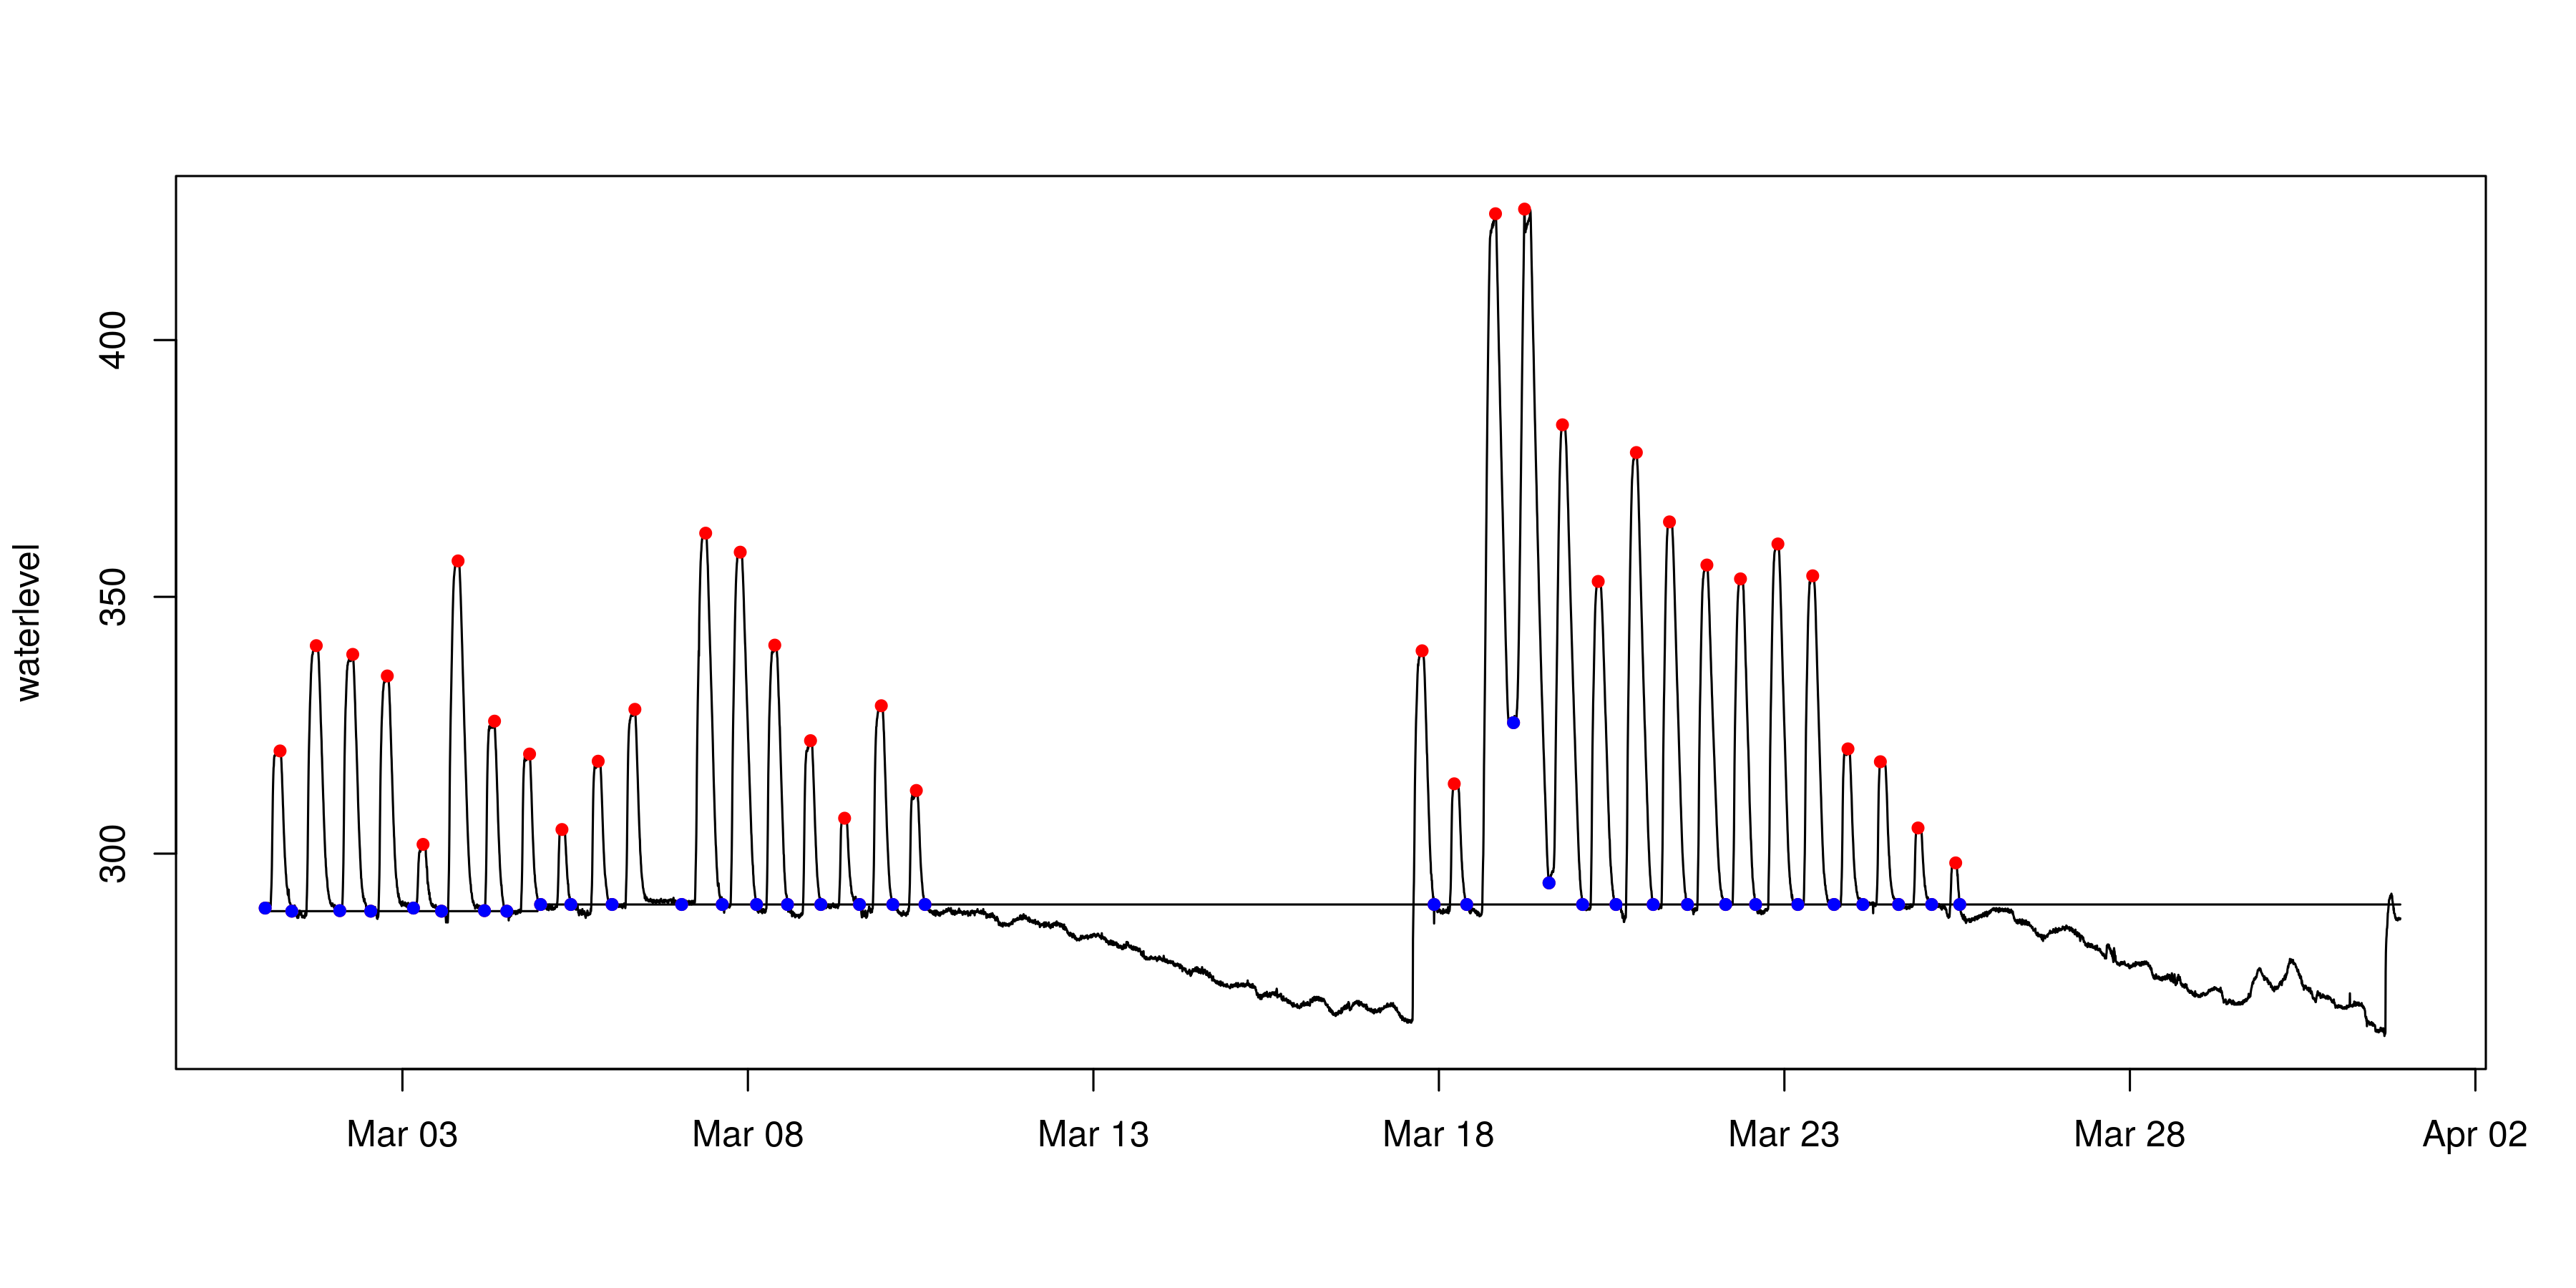
\includegraphics{Tides-TideFig3}
\end{center}
\caption{Result of simple plotting method on tides object. It plots the time series with minima and maxima added as coloured dots} 
\label{Fig3}
\end{figure}




\bibliography{Tides}
\bibliographystyle{apalike2}

\end{document}
